\documentclass{beamer}
\usepackage{HECbeamer}
% \usepackage{pgfpages}
% \pgfpagesuselayout{4 on 1}[letterpaper, landscape, border shrink=5mm]
\title[\color{white}{MATH 60604 \S~7b - Vraisemblance et analyse de survie}]{\texorpdfstring{MATH 60604 \\Modélisation statistique \\ \S~7b - Vraisemblance et analyse de survie}{MATH 60604 \\ Modélisation statistique \\ \S~7b - Vraisemblance et analyse de survie}}
\author{Léo Belzile}
\institute{HEC Montréal\\
Département de sciences de la décision}
\date{} 

\begin{document}
\frame{\titlepage}


\begin{frame}
\frametitle{Fonctions de survie et de risque} 

Soit $T$ la variable aléatoire représentant le temps de survie 
\bi %\item On dénote la fonction de répartition $F(t) = \P{T \leq t}$ et la fonction de densité $f(t) = \d F(t) / \d t$. 
\item  La \alert{fonction de survie}, $S(t) = \P{T>t}$, caractérise complètement la loi de $T$.
\item On veut souvent savoir quelles périodes présentent un plus fort taux de défaillance.
La \alert{fonction de risque} (taux de défaillance, taux de risque) de $T$ est 
\begin{align*}
h(t) &= \lim_{\delta \to 0} \frac{\P{t < T<t + \delta \mid T>t}}{\delta} 
\\&= \lim_{\delta \to 0} \frac{1}{\delta}\frac{\P{t < T < t + \delta}}{\P{T>t}} \\&= \frac{f(t)}{S(t)}
\end{align*}
On peut interpréter la fonction de risque comme étant la probabilité instantanée de ``mourir'' au temps $t$, compte tenu de la survie jusqu'au temps $t$.
\ei
\end{frame}
\begin{frame}[fragile]
\frametitle{Fonctions de survie et de risque}
\begin{center}
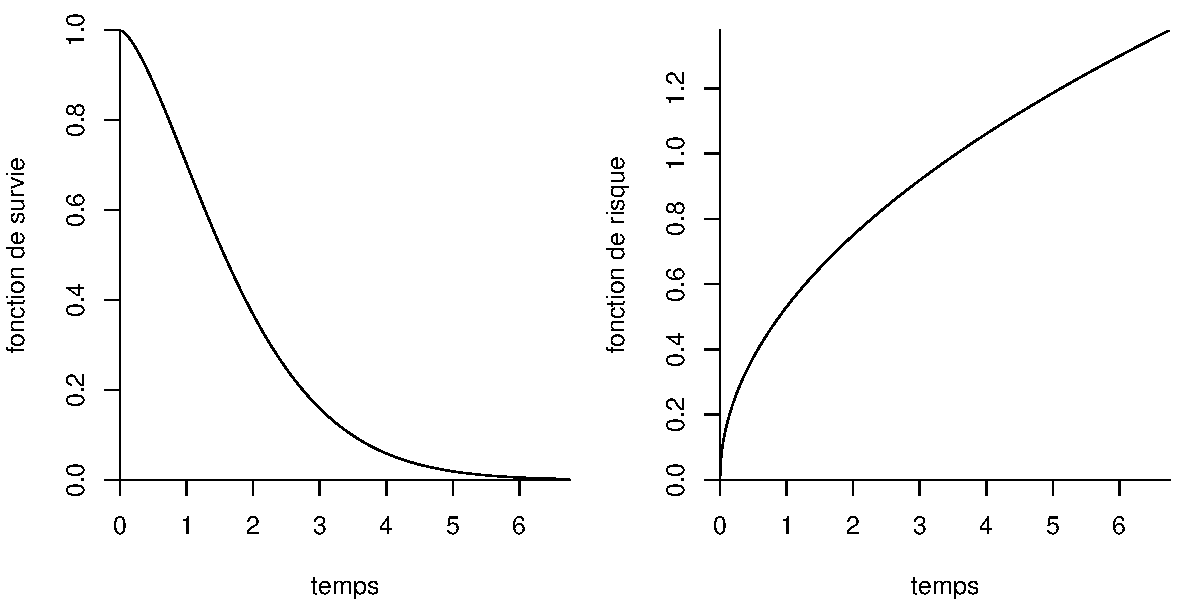
\includegraphics[width = 0.8\textwidth]{img/c7/07-survival-hazard-fr.pdf}
\end{center}
{\footnotesize

La fonction de survie décroît de $S(0)=1$ de manière monotone. Plus le risque $h(t)$ est élevé, plus la survie décroît rapidement.

}

\end{frame}

\begin{frame}
\frametitle{Fonction de risque en forme de bain}
\begin{center}
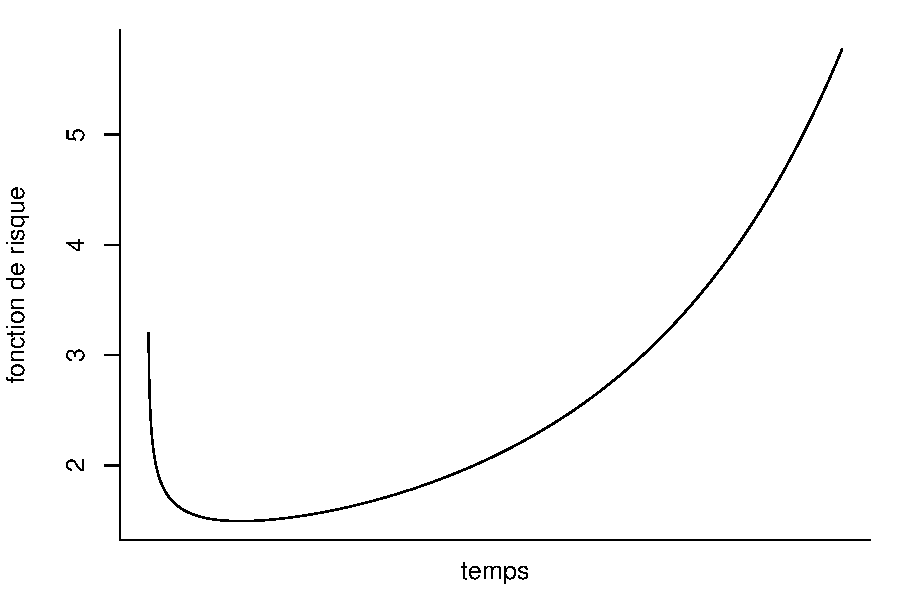
\includegraphics[width = 0.8\textwidth]{img/c7/07-bathtub-hazard-fr.pdf}
\end{center}
{\footnotesize

Le risque initial est fort (mortalité infantile, défaut de fabrication) initialement, puis décroît et se stabilise. Au fil du temps, le risque augmente de nouveau (défaillance accrue avec l'âge).

}
\end{frame}

\begin{frame}
\frametitle{Censure aléatoire et vraisemblance}
On observe $T_i = \min\{T_i^0, C_i\}$. Si une observation est censurée à droite au temps $c$, on sait que $S(c)=\P{T_i^0 > c}$
\bi \item en d'autres mots, le temps de survie excède $c$.
\ei

Si on a de la censure aléatoire, la base de données contient un indicateur $\delta_i$ où
\begin{align*}
T_i = 
\begin{cases}
T_i^0, & \delta_i=1 \text{ (événement observé)}\\
C_i, & \delta_i=0 \text{ (censure à droite)}
\end{cases}
\end{align*}
\end{frame}


\begin{frame}
\frametitle{Contribution à la vraisemblance}
Soit $S(t; \bs{\theta}) = \P{T_{i}^0 > t}$ la fonction de survie de $T_i^0$. Avec $T_i^0$ indépendant de $C_i$, chaque observation contribue 
\begin{align*}
L_i(\bs{\theta}) = 
\begin{cases} 
f(t_i; \bs{\theta}), & \delta_i=1 \text{ (événement observé)}\\
S(t_i; \bs{\theta}), & \delta_i=0 \text{ (censure à droite)}
\end{cases}
\end{align*}
à la vraisemblance. La log vraisemblance s'écrit 
\begin{align*}
\ell(\bs{\theta}) \equiv \sum_{i: \delta_i=1} \ln f(t_i; \bs{\theta}) + \sum_{i: \delta_i=0} \ln S(t_i; \bs{\theta})
\end{align*}

\end{frame}
\begin{frame}
\frametitle{Approches pour l'inférence}

Plusieurs approches s'offrent à nous pour estimer la fonction de survie (ou la fonction de risque).
\bi \item paramétrique: choisir une famille de lois (Weibull, log normale, Gompertz, exponentielle) pour $T$.
\bi
\item[$+$] permet d'incorporer des variables explicatives aisément
\item[$+$] estimés continus, permet d'extrapoler la courbe
\item[$-$] notre modèle peut être mal spécifié
\item[$-$] peu flexible: la loi peut mal s'ajuster aux données
\ei
\item nonparamétrique: aucune distribution assumée. 
\bi 
\item[$-$] pas de variables explicatives
\item[$+$] hypothèse minimales, garanties théoriques quand la taille de l'échantillon $n$ est grande.
\item[$+$] flexible.
\item[$-$] estimés discontinus,
\item[$-$] on ne peux extrapoler au delà du plus grand temps de défaillance observé.
\ei
\ei
\end{frame}


\begin{frame}
\frametitle{Modèles paramétriques pour la survie: loi exponentielle}
Soit  $T_i \simiid \mathsf{E}(\lambda)$ des variables exponentielles d'espérance $\lambda^{-1}$.
\bi \item 
La fonction de survie de $T$ est $S(T) = \exp(-\lambda t)$ et 
\item la fonction de risque $h(t)=\lambda$ est \textbf{constante}.
\ei

La log vraisemblance pour un échantillon aléatoire de taille $n$ s'écrit
\begin{align*}
\ell(\lambda) =\sum_{i=1}^n \{\delta_i \ln \lambda - \lambda T_i\}.
\end{align*}
Le maximum de vraisemblance est $\widehat{\lambda} =\sum_{i=1}^n \delta_i/ \sum_{i=1}^n T_i $. 

\bi \item L'estimé du temps de survie est infini si aucune défaillance n'est observée.
\item On obtient les erreurs-types à l'aide de la matrice d'information observée $j(\widehat{\lambda}) = \sum_{i=1}^n \delta_i/\widehat{\lambda}^2$; les données censurées ne contribuent pas d'information.
\ei

\end{frame}

% \begin{frame}
% \frametitle{Régression probit}
% \bi \item On peut utiliser l'inférence basée sur la vraisemblance plus généralement pour d'autres scénarios de survie.
% \item 
% On considère une variable latente $Z_i \sim \mathsf{No}(\mathbf{x}_i \bs{\beta}, 1)$, mais on observe
% \begin{align*}
%  Y_i = \begin{cases}
%         0 & Z_i \leq 0, \text{ (censure à gauche)}\\
%         1 & Z_i > 0  \text{ (censure à droite)}.
%        \end{cases}
% \end{align*}
% \item  On a $\P{Y_i = 0} = \P{Z_i \leq 0} = %1-\P{Z_i-\mathbf{x}_i\bs{\beta} \leq -\mathbf{x}_i\bs{\beta}}=
% \Phi(-\mathbf{x}_i\bs{\beta})=1-\Phi(\mathbf{x}_i\bs{\beta})$.
% \item Cela revient à ajuster un modèle linéaire généralisé pour des données binaires avec fonction de liaison $g(x)=\Phi^{-1}(x)$.
% \ei
% \end{frame}



\end{document}
